\documentclass[12pt]{article}
 
\newenvironment{sol}[1][Solution]{\begin{trivlist}\item[\hskip\labelsep {\bfseries #1:}]}{\end{trivlist}}
\usepackage{minted}
%\usemintedstyle{perldoc}
\usemintedstyle{vs}
\usepackage{graphicx}
\graphicspath{./}

\usepackage[margin=1in]{geometry} 
\usepackage{amsmath,amsthm,amssymb}
\usepackage{times,url}
\usepackage{tikz}
\usepackage{color}
\usepackage{enumerate}
\begin{document}
\renewcommand{\qedsymbol}{\filledbox}
\begin{center}
    \textbf{CS 5/7350 - Test\#3} \\
    \textbf{May 11, 2022}
%replace X with the appropriate number
\end{center}
\begin{flushright}
Name: \underline{Bingying Liang }\\
ID:  \underline{\ \ \ \ \ 48999397 \ \ \ \ \ }
\end{flushright}

\begin{enumerate}
    \item \ \textcolor{red}{[11 pts] Consider the following NP completeness questions. Answer them with the best answer of “some” “all” “none” or “unknown”}

    \begin{enumerate}
        \item Which Problems in NP are also in P? (“some” “all” “none” or “unknown”)
        \begin{sol}
            unknown
        \end{sol}
        \item Which Problems in P are also in NP? (“some” “all” “none” or “unknown”)
        \begin{sol}
            all
        \end{sol}
        \item Which Problems in NP-Hard are also in NP? ( “some” “all” “none” )
        \begin{sol}
            some
        \end{sol}
        \item Which Problems in NP-Complete are in NP-Hard ( “some” “all” “none” or “unknown”)
        \begin{sol}
            all
        \end{sol}
        \item If someone can solve an NP-Complete problem in Polynomial Time, then all NP and all NP-Hard problems can be solved in polynomial time. (true or false)
        \begin{sol}
            false
        \end{sol}
        \item If someone can solve an NP-Complete problem in Polynomial Time, then all NP and all NP-Complete problems can be solved in polynomial time. (true or false)
        \begin{sol}
            true
        \end{sol}
        \item At least 1 NP problem has a known solution to solve it in polynomial time? (True or False)
        \begin{sol}
            true
        \end{sol}
        \item All NP-Complete problems are in P (“true” “false” or “unknown”)
        \begin{sol}
            unknown
        \end{sol}
        \item Which NP-Hard Problems are also NP-Complete? ( “some” “all” “none” or “unknown”)
        \begin{sol}
            some
        \end{sol}
        \item To show a problem, Q, is NP-Complete, you must show Problem Q is NP and that a solver for another NP-Hard problem can solve problem Q as well. (True or False)
        \begin{sol}
            False
        \end{sol}
        \item To show a problem, Q, is NP-Complete, you must show Problem Q is NP and that a solver for problem Q can solve another NP-Hard problem. (True or False)
        \begin{sol}
            True
        \end{sol}

    \end{enumerate}

    \item \ \textcolor{red}{[6 pts] Consider an LZW compression scenario with a dictionary that contained 1024 entries. In this dictionary, entries 0-255 were the standard ASCII values and entries 256-1023 were the dynamic part of the dictionary. This compression was able to compress a file of 1000kB to 750kB:
    \begin{enumerate}
        \item What is one reason that a larger dictionary of size 2048 with dynamic entries from 256-2047 might cause the file to compress SMALLER than 750kB?
        \begin{sol}
            A larger dictionary can allow more patterns to be remembered and used without to build them again.
        \end{sol}
        \item What is one reason that a larger dictionary of size 2048 with dynamic entries from 256-2047 might cause the file to compress LARGER than 750kB
        \begin{sol}
            A larger dictionary means that more bits are needed for each symbol in the compressed message.
        \end{sol}
    \end{enumerate}
    }

    \item \ [6 pts] You have a tree with the following in-order and pre-order traversals. Draw the tree:
    \begin{align*}
        \text{IN ORDER: L V Y T X Z W P Q R M}\\
        \text{PRE\_ORDER: L P X Y V T W Z M Q R}
    \end{align*}
    \begin{sol}
    \hspace*{\fill}
                \begin{center}
    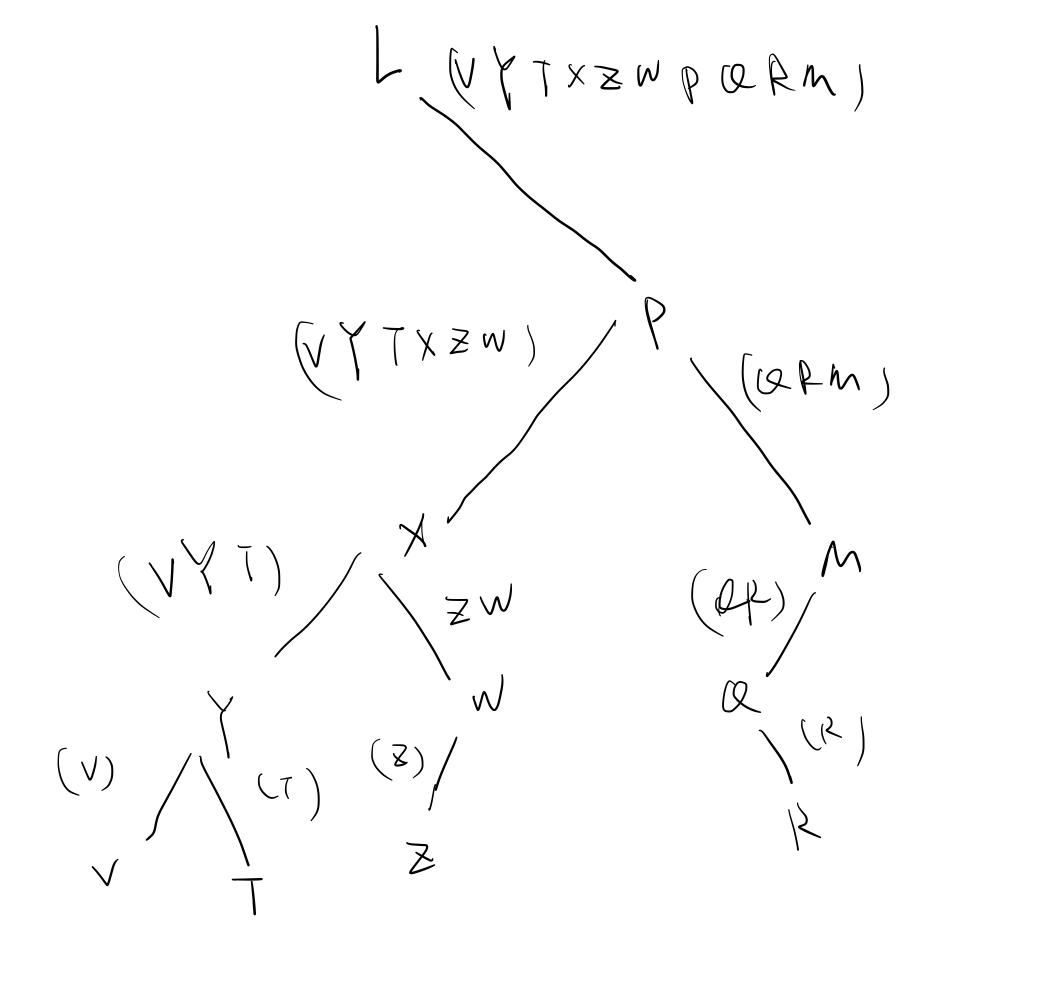
\includegraphics[width=0.6\textwidth]{p2.jpeg}
    \end{center} 
    \end{sol}

    \item \ [6 pts] You have 3 dice. Each one is different.
    \begin{itemize}
        \item Die \#1 has sides \{0, 1, 2\} with a
        \item Die \#2 has sides \{1, 2, 3\} with a 
        \item Die \#3 has sides \{0, 1\} with a
    \end{itemize}
    \begin{enumerate}
        \item Fill in the table for the dynamic programming algorithm to solve the problem.
        \begin{sol}
            \hspace*{\fill}
                            \begin{center}
    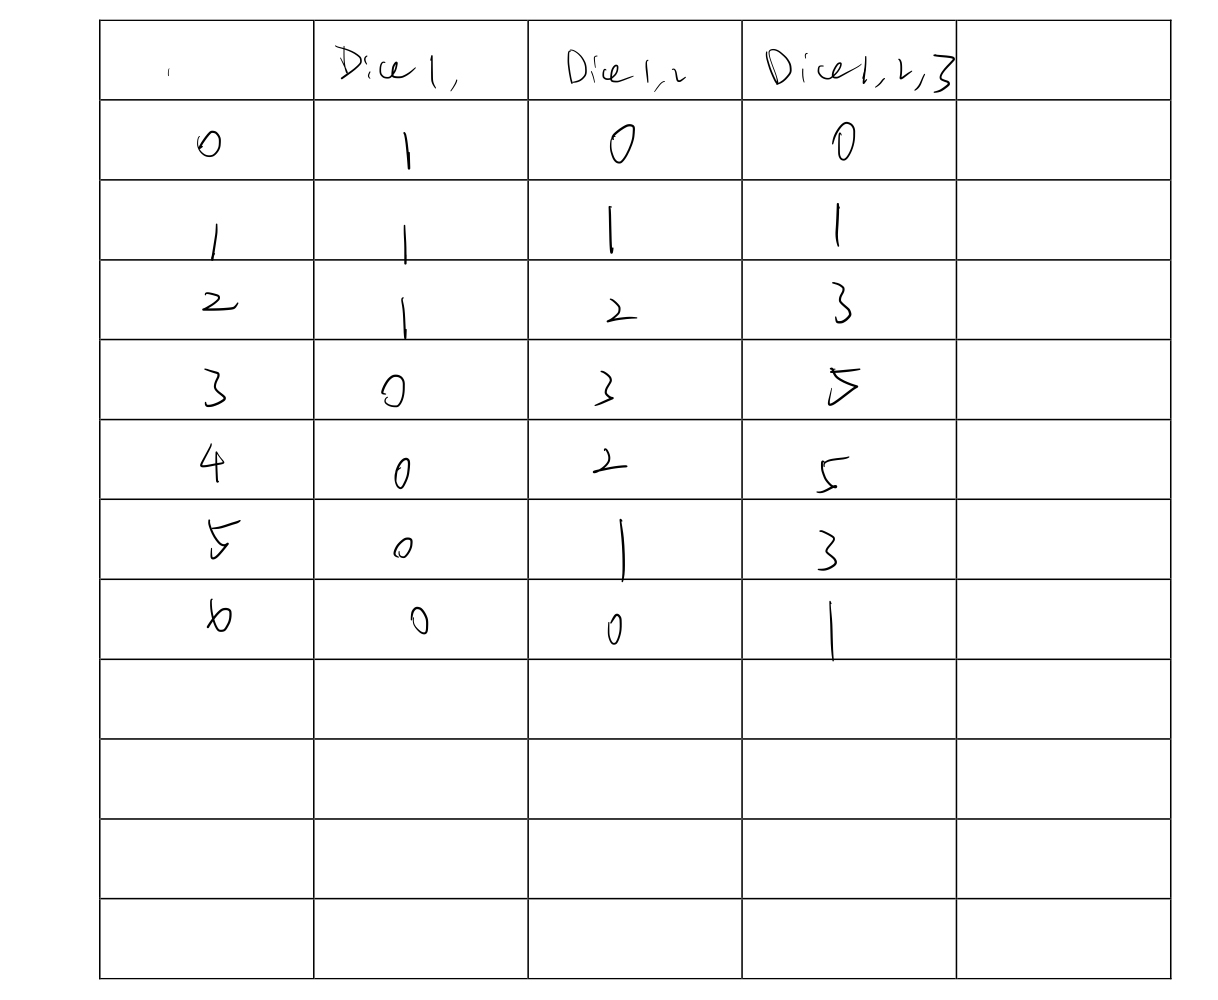
\includegraphics[width=0.4\textwidth]{p3.jpeg}
    \end{center} 
        \end{sol}
        \item What is the probability of rolling a 0?
        \begin{sol}
            0
        \end{sol}
        \item What is the probability of rolling a 3?
        \begin{sol}
        $\frac{5}{18}$
        \end{sol}
        \item What is the probability of rolling a 6?
        \begin{sol}
            $\frac{1}{18}$
        \end{sol}
    \end{enumerate}

    \item \ [6 pts] Answer the following questions.:
    \begin{enumerate}
        \item A program requires 5s to attack an encryption key of 128 bits. If the running
time is $\Theta(2^n)$ about how many years would it take to brute force attack an encryption key of 256 bits? (note there are about 32 million seconds in a year)
\begin{sol}
    \begin{align*}
        \frac{2^{256}}{2^{128}} \times 5s = 2^{128} \times 5s = 2^{128} \times 5 \times \frac{1}{32\times 10^6} \\=\frac{2^{128}}{2^5}\times 5 \times 10^{-6} = 2^{123}\times 5 \times 10^{-6} \ years
    \end{align*}
\end{sol}
\item A program requires 5s to attack an encryption key of 128 bits. If you have access to a quantum computer where the running time is $\Theta(n^2)$ about how many seconds would it take to brute force attack an encryption key of 256 bits?
\begin{sol}
    20s
\end{sol}


    \end{enumerate}

    \item \ [6 pts] Use the DGT algorithm discussed in class to determine how to represent the value 1023 using the number system $\beta$=5, D = \{ -2, -1, 0, 1, 7 \}. Show your work
    \begin{sol}
        \begin{align*}
        & -2 \bmod 5 = 3, -1 \bmod 5 = 4, 7 \bmod 5 = 2 \\
        & 1023 \bmod 5 = 3 \rightarrow -2 \\
        & 1023 - (-2) = 1025 \\
        & 1025 \div 5 = 205\\
        & ----------------\\
        & 205 \bmod 5 = 0 \\
        & 205 - 0 = 205\\
        & 205 \div 5 = 41\\
        & ----------------\\
        & 41 \bmod 5 = 1\\
        & 41 - 1 = 40\\
        & 40 \div 5 = 8\\
        & ---------------\\
        & 8 \bmod 5 = 3 \rightarrow -2\\
        & 8 -(-2) = 10\\
        & 10 \div 5 = 2 \\
        & ---------------\\
        & 2 \bmod 5 = 2 \rightarrow 7\\
        & 2 - 7 = -5 \\
        & -5 \div 5 = -1\\
        & --------------\\
        & -1 \bmod 5  =  -1\\
        & -1-(- 1) = 0\\
        \therefore \bar{1}7\bar{2}10\bar{2}
        \end{align*}
    \end{sol}

    \item \ [8 pts] You have two strings, A and B.
    \begin{itemize}
        \item String A has a length of 11.
        \item String B has a length of 8.
        \item String C has an unknown length.
        \item The Longest Common Subsequence between String A and C is 5.
    \end{itemize}
    \begin{enumerate}
        \item What is the minimum length of String C?
        \begin{sol}
        5
        \end{sol}
        \item What is the maximum length of String C?
        \begin{sol}
            infinitely 
        \end{sol}
        \item What is the minimum length of the Levensthein Edit Distance of String A and String C ?
        \begin{sol}
            6
        \end{sol}
        \item \textcolor{red}{What is the maximum length of the Levensthein Edit Distance of String A and String B?}
        \begin{sol}
            11
        \end{sol}
    \end{enumerate}

    \item \ [6 pts] A program takes 10 seconds to process a data set of 1000 items using an algorithm that is $\Theta(n^3)$. You want to process a data set of 10,000 items.

    \begin{enumerate}
        \item How long would it take to process these 100,000 items on a computer that is 5 times faster using the algorithm that is $\Theta(n^3)$?
        \begin{sol}
            $10^6\times 2s$
        \end{sol}
        \item How long would it take to process these 100,000 items if the computer is the same speed, but the algorithm is $\Theta(n^2)$ instead?
    \end{enumerate}
    \begin{sol}
        $10^5s$
    \end{sol}

    \item \textcolor{red}{[9 pts] Compute the following. Assume Graph G has $|V|$ vertices and each edge has a weight of ‘w’. Give your answers in terms of “V” and “w” as appropriate.}
    \begin{enumerate}
        \item If Graph G is a cycle, what is the maximum flow between any two vertices? 
        \begin{sol}
            2w
        \end{sol}
        \item If Graph G is complete, what is the maximum flow between any two vertices?
        \begin{sol}
            (v-1)w
        \end{sol}
        \item If Graph G is a tree, what is the maximum flow between any two vertices?
        \begin{sol}
            w
        \end{sol}
        \item If Graph G is a cycle, the value of the minimum spanning tree of graph G is?
        \begin{sol}
            (v-1)w
        \end{sol}
        \item If Graph G is complete, the value of the minimum spanning tree of graph G is?
        \begin{sol}
            (v-1)w
        \end{sol}
        \item \textcolor{red}{If Graph G is a tree, the value of the minimum spanning tree of graph G is?}
        \begin{sol}
            (v-1)w
        \end{sol}
        \item If Graph G is a cycle, for what values of $|V|$ does graph G have an Euler Tour?
        \begin{sol}
            All
        \end{sol}
        \item If Graph G is complete, for what values of $|V|$ does graph G have an Euler Tour?
        \begin{sol}
            $|V|$ is odd.
        \end{sol}
        \item If Graph G is a tree, for what values of $|V|$ does graph G have an Euler Tour?
        \begin{sol}
            None
        \end{sol}
    \end{enumerate}
    \item \ [5 pts] Argue that the problem, S, of sorting an unsorted array of integers of length greater than 100 elements is at least as hard - and maybe even harder - than the problem, L, of finding the median of the same array.
    \begin{sol}
    I can use a solver for S to solve L by sorting the array and returning the element in the middle index, since a solver for S can solve L, s must be at least as hard or possibly harder than L.
    \end{sol}

    \item \ [9 pts] A message contains the following number of each symbol:
    \begin{center}
        30 A’s, 14 B’s, 6 C's, 4 D's, 3 E's, 3 F's, 2 G's, 1 H and 1 K.
    \end{center}
    \begin{enumerate}
        \item Create a Huffman coding for each symbol:
                        \begin{center}
    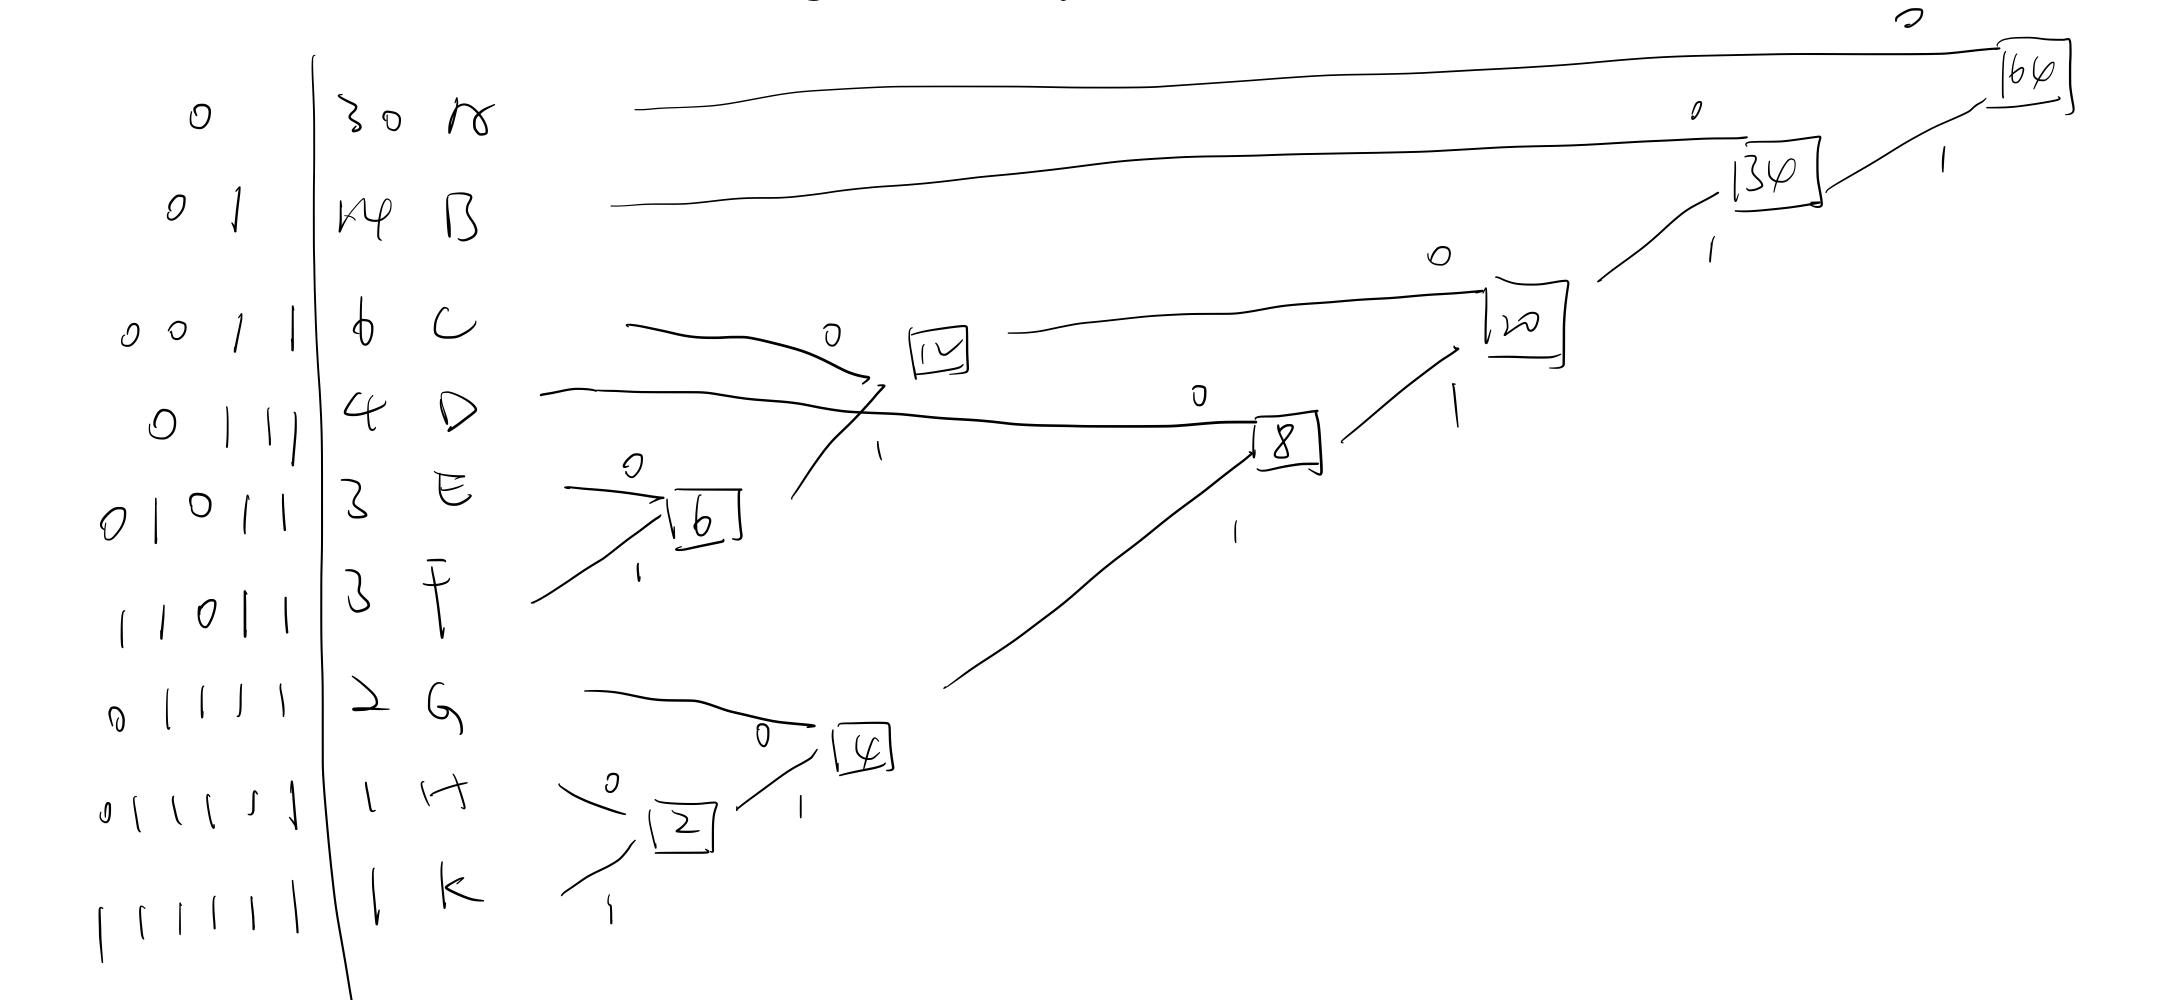
\includegraphics[width=0.9\textwidth]{p4.jpeg}
    \end{center} 
        \item How many bits are in the entire Huffman coded message?
        \begin{sol}
            150 bits
        \end{sol}
        \item How much entropy does each “C” have?
        \begin{sol}
            $\log_2(\frac{32}{3})$ bits
        \end{sol}
    \end{enumerate}

    \item \ \textcolor{red}{[6 pts] Consider the following graph. When necessary for the algorithm, use vertex C as the starting vertex:}
        \begin{center}
    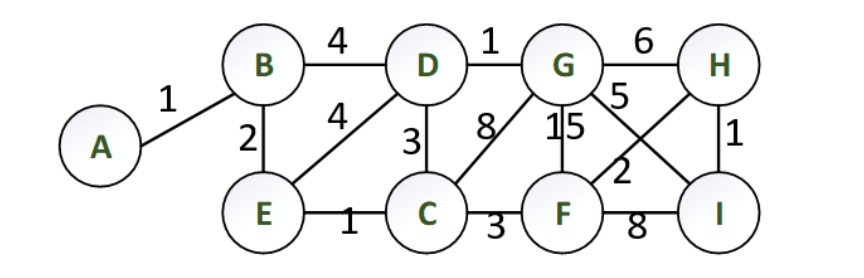
\includegraphics[width=0.4\textwidth]{p1.png}
    \end{center} 
    \begin{enumerate}
        \item Give a smallest last vertex ordering for the graph. Circle in your ordering the first vertex you wrote down for that ordering.
        \begin{sol}
        \hspace*{\fill}
                    \begin{center}
    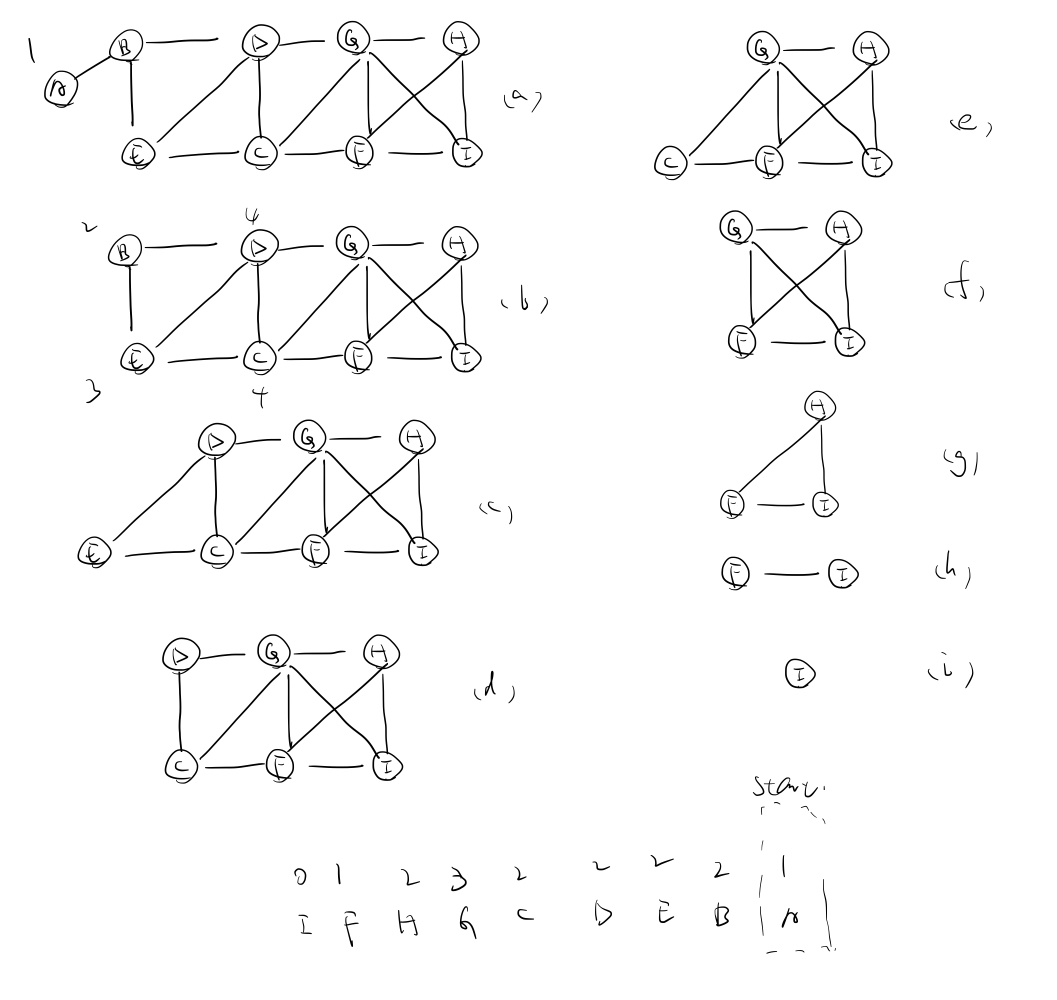
\includegraphics[width=0.8\textwidth]{p5.jpeg}
    \end{center} 
        \end{sol}
        \item What is the edge you would choose $3^{rd}$ when finding a minimum spanning tree with Kruskal’s algorithm?
        \begin{sol}
            1: EC, AB, DG, HI
        \end{sol}
        
        \item What is the edge you would choose $3^{rd}$ when finding a minimum spanning tree with Prim’s algorithm?
        \begin{sol}
            AB
        \end{sol}


    \end{enumerate}

    \item \ [4 pts] Two people need to establish a secret key for encrypting communications. They agree to use a Diffie-Hellman key exchange with a modulus of 11 and decide on 2 as the base. Person A chooses a random value performs the appropriate computations and sends the value 5 to person B. Person B chooses a random value of 3 and performs the appropriate computations:
    \begin{enumerate}
        \item What is the value Person B sends to Person A
        \begin{sol}
            8
        \end{sol}
        \item What is the shared secret key between Person A and Person B
        \begin{sol}
            4
        \end{sol}
    \end{enumerate}

    \item \ [8 pts] Consider an RSA encryption system that has a public key of 339251 for the value e and 748081 for the value of the modulus N. You also saw a message that had been encrypted by the public key. The value of this encrypted message is 2.
    \begin{enumerate}
        \item You are able to factor N=748081 into the product of two prime numbers 853 * 877. What is the value of the private key? Show your work including the table for computing the Extended Euclidean Algorithm.
        \begin{sol}
            d = 11; private(11, 748081)
        \end{sol}
        \item What was the original message before encryption? (Give an integer)
        \begin{sol}
            2048
        \end{sol}
    \end{enumerate}

    \item \ [4 pts] Using $n_0$ equal to 10, show that $f(n) = 6n^3 + 2n^2 + 4n + 1$ is $\Theta(n^3)$.
    \begin{sol}
        \begin{align*}
            \Omega(n^3): & 0 \leq c_1g(n) \leq f(n), \forall n = n_0 = 10\\
            & c_1 n^3 \leq 6n^3 + 2n^2 + 4n + 1, \forall n = n_0 = 10\\
            & c_1 \leq 6 + \frac{2}{n} + \frac{4}{n^2} + \frac{1}{n^3}, \forall n = n_0 = 10\\
            & c_1 \leq 6 + \frac{2}{10} + \frac{4}{100} + \frac{1}{1000}\\
            & \therefore c_1 = 6 \text{ can let }f(n) \text{ is } \Omega(n^3), \forall n = n_0 = 10
        \end{align*}
                \begin{align*}
            O(n^3): & 0 \leq  f(n)\leq c_2g(n), \forall n = n_0 = 10\\
            & 6n^3 + 2n^2 + 4n + 1 \leq c_2 n^3, \forall n = n_0 = 10\\
            & 6 + \frac{2}{n} + \frac{4}{n^2} + \frac{1}{n^3} \leq  c_2 , \forall n = n_0 = 10\\
            & 6 + \frac{2}{10} + \frac{4}{100} + \frac{1}{1000} \leq  c_2\\
            & 6.241 \leq c_2 \\
            & \therefore c_2 = 6.241 \text{ can let }f(n) \text{ is } O(n^3), \forall n = n_0 = 10 \\
        \end{align*}
    \end{sol}



\end{enumerate}

\end{document}
